\documentclass[10pt,a4paper]{article}
\usepackage[margin=2.2cm]{geometry}
\usepackage{graphicx,booktabs,amsmath,hyperref,caption}
\captionsetup{font=small}
\title{When is knowing the cause worth the measurement?\\\large Degradation diagnosis on the SSMR ethanol-reforming benchmark (technical note v1, draft)}
\author{Bosco Chiramel\thanks{Draft prepared with AI assistance (Claude); every number is generated by scripts in the accompanying repository and checked by a verifier script. To be rewritten by the author before any release.}}
\date{30 September 2026 --- DRAFT, not released}
\begin{document}\maketitle
\begin{abstract}\noindent
When delivered hydrogen falls in a membrane reformer, can an operator tell catalyst deactivation from membrane fouling, feed shortfall or hydrogen-meter drift, and does it matter for what they do next?
On the published SSMR benchmark (Arcila-Osorio et al., 2026), reproduced in Python and checked against the authors' code in MATLAB (largest hydrogen difference 0.0564\% of nominal), we map each cause and loss level to three regions: distinguishable, indistinguishable with the same action, and indistinguishable with a different action.
With the hydrogen flow alone none of the reachable scenarios is distinguishable, because a slow meter drift can mimic any process loss and calls for the opposite action.
A bounded six-minute feed move of +0.0003 mol/min, costing 0.0018 mol of ethanol, separates catalyst from membrane loss at a 5\% hydrogen drop by 7.0 noise standard deviations and resolves most losses of 5\% or more, while extra steady sensors without the move add less.
These are simulation results on the authors' exponential deterioration mechanisms with a declared noise model; no 1\% loss is distinguishable under any measurement set tested.
\end{abstract}

\section{Problem}
The benchmark of Arcila-Osorio, Destro, Ocampo-Martinez, Llorca and Braatz \cite{bench} provides a validated dynamic model of a two-stage staged-separation membrane reactor, six control challenges and deterioration scenarios in which all kinetic pre-factors decay as $e^{-0.01t}$ (catalyst) or the permeance pre-factor as $e^{-0.006t}$ (membrane), $t$ in minutes. The authors state that catalyst activity and membrane permeability are treated as run-invariant ``(i.e., no explicit deactivation, fouling, or aging kinetics)'' and that the release is deterministic, without sensor noise \cite{bench}. Challenge 4 notes that ``the catalyst activity is not measured''. This note works inside that stated gap. The question is a decision, not an estimation exercise: \emph{when delivered hydrogen falls, when is identifying the cause worth the measurement, and what is the least disruptive experiment that identifies it?}

\section{Prior work}
Serra, Ocampo-Martinez, Li and Llorca \cite{serra} designed linear MPC for an ethanol steam reformer with Pd-Ag membrane separation on a model fitted to the same group's experiments; they do not address degradation diagnosis. Scott, Findeisen, Braatz and Raimondo \cite{scott} and Raimondo, Marseglia, Braatz and Scott \cite{raimondo} design open- and closed-loop inputs that guarantee fault diagnosis for faults modelled as switches between linear systems with bounded uncertainty (zonotopes). The feed move below is an active-diagnosis input in their sense. What this note adds is narrower and practical: a computed map, on this nonlinear benchmark, of where the cause is identifiable from the signals an operator has, where the distinction changes the operating action, and what a one-step bounded move buys in operator units. We make no claim about optimal input design. The broader fault-diagnosis benchmark literature was not surveyed for this draft (see Limitations).

\section{Baseline reproduction (M1)}
The released MATLAB code (commit c628084) was run untouched in MATLAB R2026a for the four reference cases; only the README case settings were changed, in copies. A vectorised Python port of the same equations was compared on matched samples (Table~\ref{tab:m1}). Every approved equivalence gate passes: largest hydrogen difference 0.0564\% of nominal (gate 0.5\%), largest IAE difference 0.141\% (gate 1\%).

\begin{table}[h]\centering\small
\caption{Native MATLAB versus Python port, and MATLAB versus the paper's reported IAE.}\label{tab:m1}
\begin{tabular}{lrrrr}\toprule
case & max $\Delta$H$_2$ (\% nom.) & max $\Delta$EtOH (\% nom.) & IAE diff (\%) & MATLAB IAE vs paper \\\midrule
STEP & 0.0145 & 0.0000 & -- & -- \\
CS1 & 0.0347 & 0.0149 & 0.141 & -0.05\% \\
CS2T & 0.0564 & 0.0358 & 0.003 & -10.52\% \\
CS2P & 0.0177 & 0.0112 & 0.004 & -9.30\% \\\bottomrule
\end{tabular}\end{table}

Case study 1 reproduces the paper. The disturbance cases do not, in MATLAB either, so the difference is between the released code and the paper, not in the port. For CS2T the gap equals 0.997 times one 0.1-min sample of full set-point error at the steam-only start; this pattern was found after the comparison and is a question for the authors, not a pass. The paper's ``time constant 0.25~min'' is not what a first-order-plus-dead-time fit returns (0.050~min with 0.203~min dead time); the elapsed time from the input change to 63.2\% of the rise is close to 0.25~min. Two further findings: \texttt{control.m} keeps PID state in persistent variables that the script's \texttt{clear} does not reset, so running cases back to back moved CS1's IAE by +20.1\%; and GNU Octave's \texttt{ode15s} ignores the \texttt{NonNegative} option and cannot integrate the Mode~2 steam-only start, so Octave is not a substitute reference for Mode~2.

\section{Method (M2--M4)}
\textbf{Quasi-steady map.} Deterioration is slow against the reactor response, so steady states were computed on a grid of catalyst multiplier $a_c$, membrane multiplier $a_m$ (0.4--1) and ethanol feed (0.0018--0.0024 mol/min), 210 points, all converged, and interpolated. Gate V1: against full dynamic runs of the authors' two deterioration schedules over 20~min the map differs by at most 0.027\% (catalyst) and 0.0001\% (membrane) of nominal hydrogen (gate 0.5\%). Gate V2: held-out points differ by at most 0.00002\%. (Figure~\ref{fig:v1}.)

\textbf{Measurement layer.} Declared scenario values, not instrument specifications: hydrogen flow noise 0.5\% of nominal with an unknown constant bias of up to 0.5\%; outlet temperature 0.5~K noise, 1~K bias; waste-gas flow 1\%/2\%; micro-GC mole fractions of H$_2$, CH$_4$, CO, CO$_2$ at 1\% relative noise, 2\% bias, every 3~min with 3~min delay; a 10-min decision window. Measurement sets: S1 = H$_2$ flow; S2 = + outlet temperature; S3 = + waste flow; S4 = + mole fractions; ``+E'' adds the feed move (+0.0003 mol/min held 5~min after 1~min settling).

\textbf{Hypotheses and test.} Catalyst loss, membrane loss, feed shortfall (delivered ethanol a fraction of the command) and additive hydrogen-meter drift, each with one scalar severity, set to give 1, 2, 5, 10 or 20\% hydrogen drop at the mode's nominal feed. For each alternative cause the severity that best explains the data is fitted; its bias-robust statistic $\Lambda$ is compared with a $\chi^2_{0.99}$ threshold. The frozen protocol used $k-1$ degrees of freedom; because this penalises larger sensor sets, a dated amendment (A1) with one degree of freedom is reported beside it. Local structural identifiability: the noise-scaled sensitivity matrix has rank 2 for S1+E and 4 for S4+E in Mode~1 (four parameters).

\textbf{Actions.} For a process loss, the operator raises ethanol to restore the set-point if that is feasible within the 0.0024~mol/min bound; otherwise the component must be serviced. For meter drift, the action is to recalibrate and not change the feed. Costs of acting on the wrong cause are hydrogen shortfall or wasted ethanol, in mol/min.

\section{Results}
\textbf{Worked ambiguity case (M3).} In Mode~1 at 0.0021~mol/min, catalyst activity 0.673 and membrane factor 0.949 both give a 5\% hydrogen drop. Hydrogen, outlet temperature and waste flow differ by less than the bias bound; methane mole fraction differs by 2.1 noise units after bias. After the feed move, the hydrogen response differs by 7.0 standard deviations of the measured difference; $\Lambda$ for the wrong cause is 36.3 (truth catalyst) and 45.3 (truth membrane), above the threshold of 6.63, so the stopping rule declares the right cause after 5~min for every measurement set (Figure~\ref{fig:m3}). Over 30~min, the authors' catalyst schedule $e^{-0.01t}$ produces the same hydrogen signal as a membrane decaying at only 0.0013/min: hydrogen here is far more sensitive to the membrane than to the catalyst, which is why the catalyst cannot reach a 20\% hydrogen drop inside the tested range.

\textbf{Operating map (M4).} Table~\ref{tab:map} counts the reachable scenarios (four causes, five loss levels) per set. With S1 no scenario is distinguishable in either mode, under either threshold. The feed move is what changes the picture (Figure~\ref{fig:map}). No 1\% loss is distinguishable under any set or threshold. Under A1 with halved or doubled noise, S1+E distinguishes 22 and 12 of the 31 reachable scenarios across both modes (16 at nominal noise).

\begin{table}[h]\centering\small
\caption{Reachable scenarios that are distinguishable (D) or indistinguishable with a different action (X), frozen threshold and amendment A1.}\label{tab:map}
\begin{tabular}{llrrrrr}\toprule
mode & set & $n$ & D frozen & X frozen & D (A1) & X (A1) \\\midrule
1 & S1 & 19 & 0 & 19 & 0 & 19 \\
1 & S1+E & 19 & 11 & 8 & 11 & 8 \\
1 & S2 & 19 & 0 & 19 & 0 & 19 \\
1 & S2+E & 19 & 9 & 9 & 11 & 8 \\
1 & S3 & 19 & 1 & 17 & 2 & 17 \\
1 & S3+E & 19 & 8 & 10 & 12 & 7 \\
1 & S4 & 19 & 3 & 16 & 5 & 14 \\
1 & S4+E & 19 & 8 & 11 & 12 & 7 \\
2 & S1 & 12 & 0 & 12 & 0 & 12 \\
2 & S1+E & 12 & 5 & 2 & 5 & 2 \\
2 & S2 & 12 & 0 & 12 & 0 & 12 \\
2 & S2+E & 12 & 4 & 4 & 5 & 2 \\
2 & S3 & 12 & 0 & 12 & 0 & 12 \\
2 & S3+E & 12 & 4 & 4 & 5 & 2 \\
2 & S4 & 12 & 0 & 12 & 0 & 12 \\
2 & S4+E & 12 & 4 & 5 & 6 & 2 \\
\bottomrule\end{tabular}\end{table}

\textbf{Value of information (Figure~\ref{fig:voi}).} Averaged over the scenarios, and relative to S1, the feed move avoids 20.9~$\mu$mol/min of wasted ethanol and 2.1~$\mu$mol/min of hydrogen shortfall in Mode~1 (A1), and 12.8 and 4.6~$\mu$mol/min in Mode~2. The move itself costs 0.0018~mol of ethanol, repaid in about 86~min of avoided waste in Mode~1. Adding waste flow and mole fractions without the move avoids 5.8~$\mu$mol/min in Mode~1: the move is worth more than the extra sensors.

\section{What to measure next on the rig}
On the authors' Pd-Ag rig: at steady operation, record permeate hydrogen (Bronkhorst meter) for 10~min, step ethanol by +0.0003~mol/min for 6~min, return. Predicted responses under each cause come from \texttt{diag/m3\_case.py}. Declare catalyst or membrane loss when exactly one hypothesis survives the $\Lambda$ test; if both survive, repeat with a 10-min hold; if both still survive, report ``deteriorated, cause not established''. Recalibrating the hydrogen meter against the soap-bubble retentate balance before the move removes the drift hypothesis, which is the most costly confusion in the map.

\section{Limitations (a hostile reviewer's list)}
\begin{enumerate}\itemsep0pt
\item \emph{Simulation only.} No experimental data; the deterioration laws are the authors' scenarios, not lifetime models. Conceded.
\item \emph{Noise and bias values are declared, not measured.} Sensitivity at $\times0.5$ and $\times2$ is reported; instrument data would replace them.
\item \emph{Quasi-steady approximation.} Checked against full dynamics (V1) for Mode~1 only.
\item \emph{Threshold choice.} The frozen rule penalises extra sensors; A1 is post-hoc. Both are shown; the main conclusions hold under both.
\item \emph{Paper mismatch.} CS2T/CS2P and the time constant do not match the paper, in MATLAB too; the author questions are open.
\item \emph{Single faults, np = 50, Modes 1--2.} Simultaneous faults, the fine grid and Mode~3 are not covered.
\item \emph{Related work.} Only the four papers cited were read; a wider fault-diagnosis sweep is pending.
\item \emph{Estimator and controller} (M6, M7) are first versions in the repository, not part of this note's claims.
\end{enumerate}

\section*{Reproducibility}
One command rebuilds every number (\texttt{run\_all.py}); protocols are frozen and hashed before results; \texttt{verify\_note.py} asserts every number in this note against the output files. Upstream code: MIT licence.

\begin{thebibliography}{9}\small
\bibitem{bench} M.~Arcila-Osorio, F.~Destro, C.~Ocampo-Martinez, J.~Llorca, R.~D.~Braatz, A benchmark simulator for advanced control of ethanol steam reforming, Renewable Energy 256 (2026) 124743, doi:10.1016/j.renene.2025.124743. Code: github.com/arcmateo/SSMR\_Benchmark.
\bibitem{serra} M.~Serra, C.~Ocampo-Martinez, M.~Li, J.~Llorca, Model predictive control for ethanol steam reformers with membrane separation, Int.\ J.\ Hydrogen Energy 42 (2017) 1949--1961, doi:10.1016/j.ijhydene.2016.10.110.
\bibitem{scott} J.~K.~Scott, R.~Findeisen, R.~D.~Braatz, D.~M.~Raimondo, Input design for guaranteed fault diagnosis using zonotopes, Automatica 50 (2014) 1580--1589.
\bibitem{raimondo} D.~M.~Raimondo, G.~R.~Marseglia, R.~D.~Braatz, J.~K.~Scott, Closed-loop input design for guaranteed fault diagnosis using set-valued observers, Automatica 74 (2016) 107--117.
\end{thebibliography}

\clearpage
\begin{figure}[h]\centering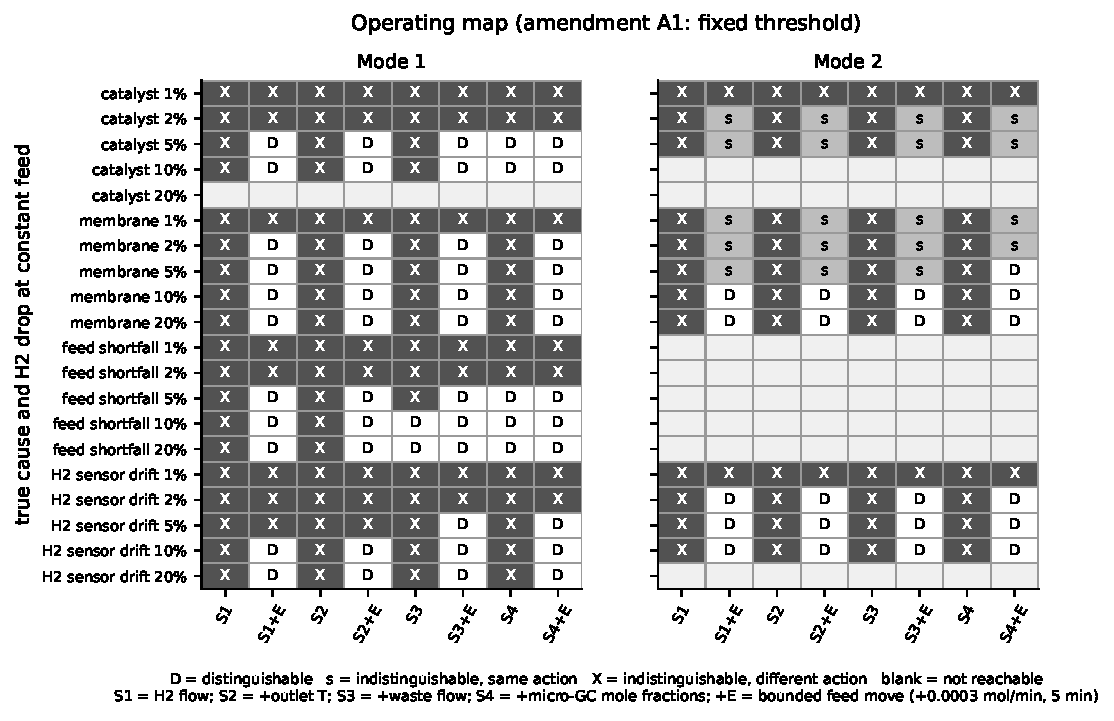
\includegraphics[width=.95\linewidth]{fig_operating_map_A1.pdf}\caption{Operating map, amendment A1 (fixed threshold). The frozen-threshold map is \texttt{fig\_operating\_map.pdf} in the repository.}\label{fig:map}\end{figure}
\begin{figure}[h]\centering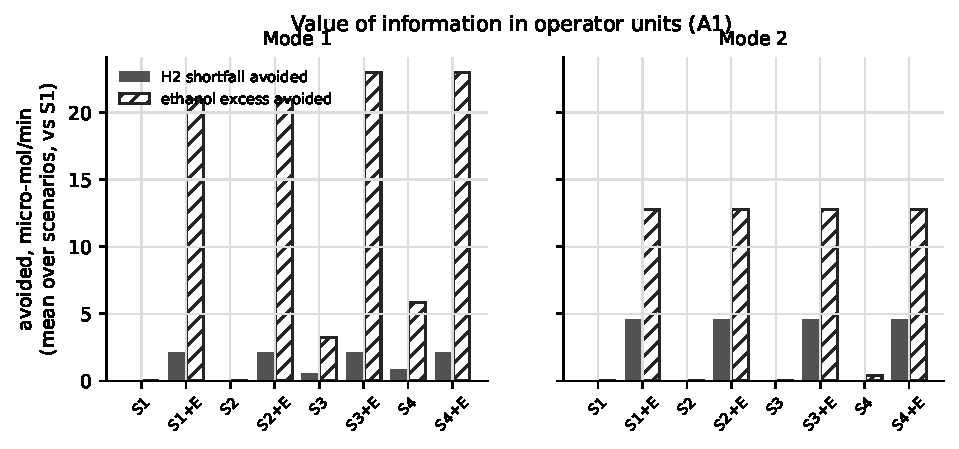
\includegraphics[width=.9\linewidth]{fig_voi_A1.pdf}\caption{Value of information relative to hydrogen flow alone (A1).}\label{fig:voi}\end{figure}
\begin{figure}[h]\centering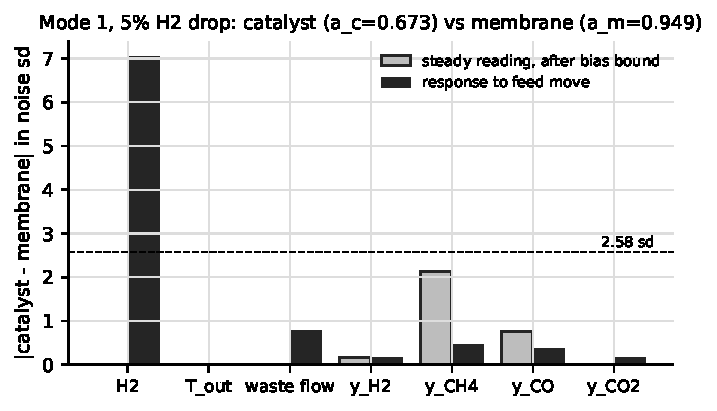
\includegraphics[width=.62\linewidth]{fig_m3_residuals.pdf}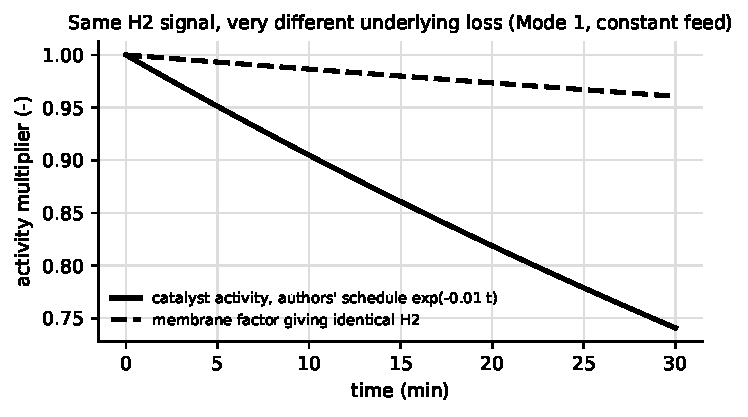
\includegraphics[width=.62\linewidth]{fig_m3_timeview.pdf}\caption{Worked case: catalyst versus membrane at a 5\% hydrogen drop.}\label{fig:m3}\end{figure}
\begin{figure}[h]\centering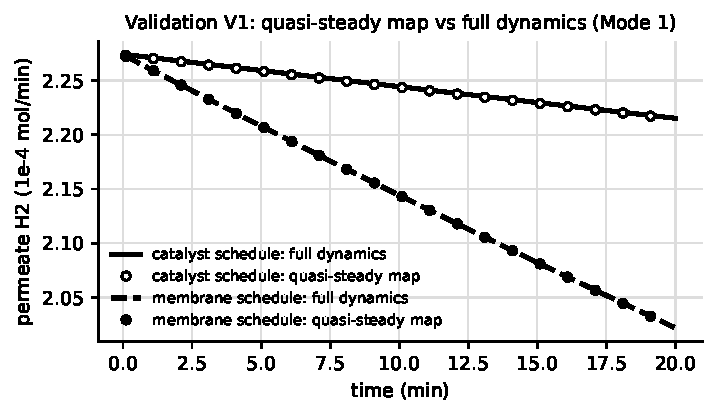
\includegraphics[width=.62\linewidth]{fig_v1_validation.pdf}\caption{Validation V1.}\label{fig:v1}\end{figure}
\end{document}
